\documentclass[11pt]{article}

\usepackage[utf8]{inputenc} % Required for inputting international characters
\usepackage[T1]{fontenc} % Output font encoding for international characters
\usepackage{graphicx}
\usepackage{float}
\usepackage{hyperref}
\usepackage{amsmath}
\usepackage{cite}
\usepackage{pdfpages}
\usepackage[german]{varioref}
\usepackage{mathpazo} % Palatino font
\usepackage[german]{babel}
\parindent0pt
\pdfinclusioncopyfonts=1

\begin{document}

\begin{titlepage} % Suppresses displaying the page number on the title page and the subsequent page counts as page 1
	\newcommand{\HRule}{\rule{\linewidth}{0.5mm}} % Defines a new command for horizontal lines, change thickness here
	
	\center % Centre everything on the page
	\vspace*{0.75cm}
%
\includegraphics[width=0.8\textwidth]{../tex/fu_logo}\\[1cm] 

%\textsc{\LARGE  Freie Universität Berlin}\\[1.5cm] % Main heading such as the name of your university/college
	
	\textsc{\Large Neurobiologie für BioinformatikerInnen: Praktikum B}\\[0.65cm] % Major heading such as course name
	
	\textsc{\large Protokoll zum 2. Praktikumstag am 14.01.2019}\\[0.65cm] % Minor heading such as course title

	\HRule\\[0.5cm]
	
	{\huge\bfseries Erregungsleitung im Bauchmark des Regenwurms}\\[0.3cm] % Title of your document
	
	\HRule\\[0.75cm]
	\textsc{\Large\bfseries Gruppe IV}
	\\[0.8cm]
	
\vfill

	\begin{minipage}{0.45\textwidth}
		\begin{flushleft}
			\large
			\textit{Gruppenmitglieder}\\
			\textsc{Alia Rothkegel}\\
			\textsc{Mara Steiger}
			 % Your name
		\end{flushleft}
	\end{minipage}
	~
	\begin{minipage}{0.45\textwidth}
		\begin{flushright}
			\large \vspace{16pt}
			alia.rothkegel@fu-berlin.de\\
			mara.steiger@fu-berlin.de 
		\end{flushright}
	\end{minipage}
	
\vfill

	\begin{minipage}{0.45\textwidth}
		\begin{flushleft}
			\large
			\textit{Lehrveranstalter}\\
			Prof. Dr. P.R. \textsc{Hiesinger}\\ 
			Dr. D. \textsc{Malun}\\ 
			Prof. Dr. M. \textsc{Wernet}
		\end{flushleft}
	\end{minipage}
	~
		\begin{minipage}{0.45\textwidth}
		\begin{flushright}
			
		\end{flushright}
	\end{minipage}
\vfill
	\begin{minipage}{0.7\textwidth}
		\begin{flushleft}
			\large
			\textit{TutorInnen}\\
			\textsc{Lisa Peters}\\
			\textsc{Johannes Brüner Hammacher}\\
			\textsc{Claudia Haushalter}
		\end{flushleft}
	\end{minipage}
	~
		\begin{minipage}{0.2\textwidth}
		\begin{flushright}
			
		\end{flushright}
	\end{minipage}

	% If you don't want a supervisor, uncomment the two lines below and comment the code above
	%{\large\textit{Author}}\\
	%John \textsc{Smith} % Your name
	\vfill\vfill\vfill % Position the date 3/4 down the remaining page

	
	\vfill % Push the date up 1/4 of the remaining page
	
\end{titlepage}

%----------------------------------------------------------------------------------------
\section{Einleitung}
Ziel der heutigen Experimente ist es, die Erregunsleitung und Funktionsweise der dorsalen Riesenaxone des Regenwurmes zu untersuchen. 

\subsection{Erregunsleitung in Nervenzellen}
Die Fortleitung von Informationen wird von Zellen des Nervensystem übernommen und basiert auf Spannungsunterschieden zwischen dessen Zellinnerem und dem extrazellulären Raum. \\
Aufgrund der Semipermeabilität der Membran von Neuronen, liegt ein sogenanntes Ruhepotential von ca. -70mV vor. Die Membran ist für größere Ionen wie Natrium ($Na^{2+}$) nicht permeabel, aber Kalium ($K^{+}$) kann frei diffundieren. Durch die geringere Konzentration von Kalium-Ionen im Zellinneren, kommt es zu einem Kalium-Austrom d.h. einem Austrom von Kationen, sodass die Nervenzelle gegenüber der Außenseite negativ geladen ist. Außerdem trägt eine Natrium-Kalium-Pumpe ($Na^{2+}$-$K^+$-ATPase) zum Erhalt des Membranpotentials bei.  \\
Eine Nervenzelle wird durch die Bindung eines Neurotransmitters an einen ligandengesteuerten Ionenkanal in der Plasmamembran aktiviert. Dieser Kanal öffnet sich durch die Bindung, woraufhin $Na^{2+}$ und $Ca^{2+}$ entlang des Konzentrationsgradienten in die Zelle einströmen und eine Depolarisation bewirken. Spannungsabhängige $Na^{2+}$-Kanäle entlang des Axons einer Nervenzelle, die durch die Depolarisation in benachbarten Regionen der Zelle kurz geöffnet werden, sorgen für die Ausbreitung des Aktionspotentials in Form einer Depolarisationswelle durch das Neuron. Kurz nach der Depolarisation durch Natrium-Einstrom öffnen sich auch spannungsgesteurte $K^+$-Kanäle entlang des Axons, die wiederum eine Repolarisation durch den Austrom von Kalium bewirken. Da diese Kalium-Kanäle etwas langsamer schließen, kommt es zu einer Hyperpolarisation der Zelle. Anschließend wird das Ruhepotential durch Leckströme von Ionen und die Aktivität der Natrium-Kalium-Pumpe wiederhergestellt.  \cite{lehninger}
\begin{figure}[H]
\makebox[\textwidth][c]{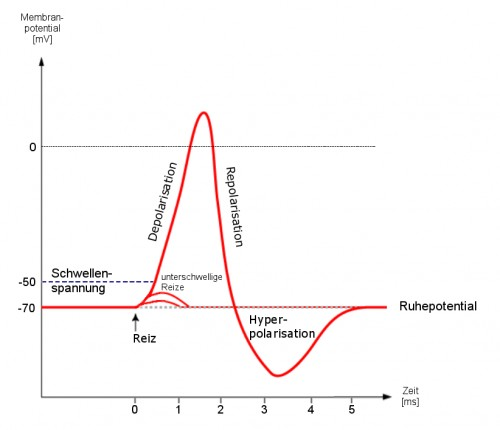
\includegraphics[width=0.85\textwidth]{aktionspotential}}
\caption{Die Abbildung zeigt den zeitlichen Verlauf eines Aktionspotentials einer Nervenzelle. Zu sehen ist die Depolarisation von -70mV auf ca. +20mV, danach die Repolarisation übergehend zur Hyperpolarisation zu ca. 100mV und die Wiederherstellung des Ruhepotentials.  }
\label{ap}
\end{figure}

Die passiven elektrischen Eigenschaften der Nervenzelle beeinflussen hierbei die Geschwindigkeit, mit der sich ein Aktionspotential ausbreitet. Dies ist zum einen der Membranwiderstand $R_m$, zum anderen die Membrankapazität $C_m$ und außerdem der intrazelluläre Längswiderstand $R_i$. Außerdem wirkt sich der Durchmesser eines Neurons auf die Fortleitungsgeschwindigkeit aus.  \cite{haustiere} 

\subsection{Refraktärphase}
Nachdem die Natrium-Kanäle während der Depolarisation kurz geöffnet waren, sind sie für eine bestimmte Zeit inaktiviert. Diese Phase nennt man Refraktärphase, währenddessen können diese Natrium-Kanäle nicht aktiviert werden und ein weiteres Aktionspotential auslösen. Dadurch wird erreicht, dass sich die Depolarisationswelle, d.h. das Aktionspotential nur in eine Richtung entlang des Axons ausbreitet.  \cite{zellbiologie} \\
Man unterscheidet zwischen der absoluten und relativen Refraktärphase. Während der absoluten Refraktärphase ist eine Erregung überhaupt nicht möglich, auch nicht durch eine starke Depolarisation. \\
Die relative Refraktärphase beginnt direkt nach der absoluten Refraktärphase. Hier ist eine erneute Erregung zwar möglich, aber das Schwellenpotential ist deutlich höher. Das heißt, um erneut ein Aktionspotential auszulösen ist ein stärkerer Reiz nötig. Außerdem ist während dieser Zeit die Amplitude des resultierenden Aktionspotentiales verringert. \cite{physiologie}

\subsection{Riesenaxone}
Die Entwicklung von Axonen mit deutlich größerem Durchmesser ist durch den evolutionären Vorteil entstanden, dass diese Aktionspotentiale schneller fortleiten können. Besonders für Bewegungsabläufe, die bei Fluchtreaktionen von Bedeutung sind, ist diese Eigenschaft entscheidend. \\
Bei der Vergrößerung des Durchmessers von Nervenfasern kommt es zu einem geringeren cytoplasmatischen Längswiderstand $R_i$, der wiederum für einen Anstieg der Längskonstante verantwortlich ist. Der Längswiderstand lässt sich wie folgt berechnen:
\begin{equation}
\label{eq1}
R_i = \dfrac{R_m}{\pi d^2}
\end{equation}
Daraus folgt, dass bei gleichem Membranwiderstand $R_m$ die Längskonstante $R_i$ für einen steigenden Durchmesser sinkt. Ursache dafür ist, dass durch den größeren Durchmesser der Widerstand, der sich in der Zelle dem Stromfluss (einströmenden Ionen) entgegenstellt, geringer ist. \\
Die Längskonstante $\lambda$ ist die Strecke, in der die maximale Amplitude der Spannungsänderung durch die Depolarisation auf den Anteil $\frac{1}{e} \approx 37\%$ abgefallen ist.  \cite{physiologie} Sie berechnet sich folgendermaßen:
\begin{equation}
\label{eq2}
\lambda = \dfrac{d/2 \cdot R_m}{2 R_i} = \dfrac{d \cdot R_m}{4 R_i}
\end{equation}
Demnach kann das Aktionspotential eine größere Distanz überbrücken, bis es seine Amplitude verliert, wenn der Durchmesser des Axons größer ist. \\
Diese Eigenschaften führten zur positiven Selektion von Riesenfasern, die man heute noch bei Arten der Bilateria finden kann. 

\subsection{Myelinisierung}
Um den Längswiderstand $L_i$ zu erhöhen, kann auch der Membranwiderstand $R_m$ bei gleichbleibendem Durchmesser $d$ vergrößert werden (\vref*{eq1}). \\
Dies wird bei der Myelinisierung über eine saltatorische Erregungsleitung erreicht, bei der im Gegensatz zu nichtmyelinisierten Axonen die aktiven und passiven Leitungsmechanismen zeitlich und räumlich voneinander getrennt sind. \\
Gliazellen umhüllen Axone und bilden die Myelinscheide, indem sie sich um die Nervenfaser wickeln. Dadurch wird das Axon isoliert und es liegt ein größerer Membranwiderstand vor, sodass der Längswiderstand verringert wird und schließlich eine Erhöhung der Längskonstante bewirkt wird (\vref*{eq2}). \\
Die myelinisierten Nervenfasern weisen sogenannte Ranvier-Schnürringe auf, an denen die aktiven Leitungsprozesse (langsamere Erregunsleitung) ablaufen , während die passiven in den isolierten Abschnitten (schnelle Erregungsleitung) erfolgen. An diesen Schnürringen liegt das Axon unmyelinisiert vor, diese kurzen Abschnitte dienen zur Regeneration der Amplitude des Aktionspotentials. \cite{physiologie}

\begin{figure}[H]
\makebox[\textwidth][c]{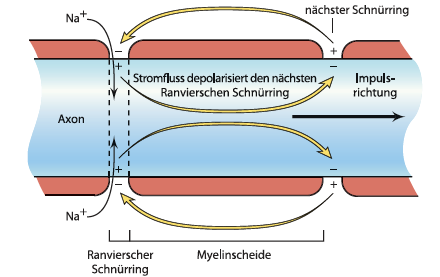
\includegraphics[width=0.85\textwidth]{myelin}}
\caption{Dies ist eine schematische Darstellung einer myeliniserten Nervenfaser. Gezeigt ist, wie ein Aktionspotential von einem zum nächsten Schnürring \glqq springt\grqq{}. }
\label{myelin}
\end{figure}


\subsection{Anatomie des Lumbricus terrestris}
Der gemeine Regenwurm (auch: Tauwurm) \textit{Lumbricus terrestris} besitzt einen länglichen bräunlich rot gefärbten Körper, der in mehrere Segmente unterteilt ist. Zur Fortbewegung befinden sich an jedem dieser Segmente zwei Borstenpaare an der Unterseite. Das vordere Ende weist eine dunklere eher braune Färbung auf und läuft spitz zu, während das hintere Ende eher heller gefärbt ist. Der Körper des Regenwurms besteht aus einer flüssigkeitsgefüllten sekundären Leibeshöhle oder \textit{Coelom} \citation{koerperbau}, die von einem formgebenden Hautmuskelschlauch umgeben ist. In der Leibeshöhle befinden sich auch die Organe des Regenwurms, sprich der Darm, die Gonaden, die Nephriden, das Ringgefäß mit Rücken- sowie Bauchgefäß und das für diesen Versuch relevante Bauchmark \ref{bauchmark}. 
\begin{figure}[H]
\makebox[\textwidth][c]{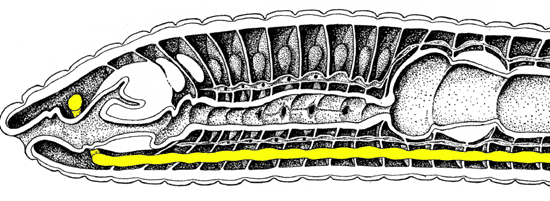
\includegraphics[width=0.7\textwidth]{bauchmark-laengs}\hspace*{4mm}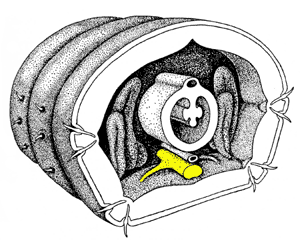
\includegraphics[width=0.35\textwidth]{bauchmark-quer}}%\makebox[\textwidth][c]{}
\caption{Eine Skizze der Anatomie des Regenwurms. Links im Längs-, rechts im Querschnitt. Das Bauchmark ist gelb hervorgehoben}
\label{bauchmark}
\end{figure}
Im Bauchmark befinden sich die Riesenfasern des Regenwurms, die mediane Riesenfaser (im Folgenden als MRF bezeichnet) und die lateralen Riesenfasern (im Folgenden als LRF bezeichnet). Zusätzlich zu dem vergrößerten Durchmesser der in ihnen liegenden Neuronen sind die Riesenfasern myelinisiert. Die beiden LRF mit je einem Durchmesser von ca. $50 \mu m$, der zu anterior abnimmt, sind über Querbrücken verbunden und fungieren so wie eine einzelne Nervenfaser. Die MRF hat einen Durchmesser von ca. $75 \mu m$, der Richtung posterior abnimmt. Sie erfüllen unterschiedliche Funktionen, und sprechen so unterschiedliche sensorische und motorische Neuronen an. Die MRF sorgt bei Reizen am anterioren Pol für das Abflachen des posterioren Körperendes und somit für ein Zurückziehen des anterioren Körperendes. Die LRF sorgen bei einem Reiz am posterioren Ende, dafür dass sich der Wurm am anterioren Ende "{}festhält"{} und das posteriore Ende wegzieht.\cite{skript}

\subsection{Differentielle Ableitung}
Eine differentielle Ableitung ist eine Methode zur Ableitung elektrischer Muskelpotentiale, bei der eine lokale Differenz zwischen zwei Elektroden gemessen wird. Dies dient dem herausfiltern von Störsignalen der elektromagnetischen Wechselfeldern der Umwelt. Es wird angenommen, dass sich diese Störsignale ca. mit Lichtgeschwindigkeit ausbreiten und somit beide Elektroden zur gleichen Zeit erreichen. Berechnet man nun die Differenz der von den Elektroden jeweils gemessenen Spannungen, so ergibt sich folgende Gleichung:
\begin{center}
$U_{ges}= (U_1+S_1) - (U_2 + S_2)$ \\

Unter der Annahme, dass $S_1 \approx S_2$, gilt: \\

$U_{ges} \approx U_1 - U_2$
\end{center}




\section{Material und Methoden}
\subsection{Material}
Für den durchgeführten Versuch wurde ein Regenwurm der Art Lumbricus terrestris als Versuchstier verwendet. Zudem eine Wurmplatte mit einer Vertiefung für das Versuchstier, sowie 2 Paaren von fest verankerten Elektroden, ein Reizgenerator, ein Verstärker, ein AD-Wandler und ein Laptop. Für die Erhebung der Daten wurde die Software Spike2 benutzt.
\subsection{Versuchsaufbau}
Für den Versuch wurde zuerst der Regenwurm unter fließendem Wasser abgewaschen und anschließend abgetrocknet.\\
Für Teil 2-4 des Versuchs wurde die Vertiefung der Wurmplatte auf einer Seite mit Knete blockiert und das Versuchstier animiert in diese hineinzukriechen. Sobald der Regenwurm sich vollständig zusammengezogen hat und mit dem vorderen Ende an der Knete und dem Körper über dem vorderen Elektronenpaar gelegt hat, wurde die Vertiefung auch hinten mit Knete blockiert und der Wurm zusätzlich mit Plexiglasplatten fixiert.\ref{foto} \\
An die Elektroden am anterioren Ende (im Folgenden "{}anteriore Elektroden"{} genannt) des Versuchstiers wurde der Reizgenerator angeschlossen und die Elektroden am posterioren Ende (im Folgenden "{}posteriore Elektroden"{} genannt) wurden mit dem Verstärker verknüpft. Sowohl der Reizgenerator als auch der Verstärker wurden über den AD-Wandler an den PC angeschlossen \ref{schema}
\begin{figure}[H]
\makebox[\textwidth][c]{\includegraphics[width=0.8\textwidth]{IMG_6360}}
\caption{Das Bild zeigt, wie der Regenwurm in der Wurmplatte mit Knete und den Plexiglasplatten fixiert wurde. Außerdem sieht man die Verkabelung der Elektroden am posterioren Ende des Wurmes. }
\label{foto}
\end{figure}
\begin{figure}[H]
\makebox[\textwidth][c]{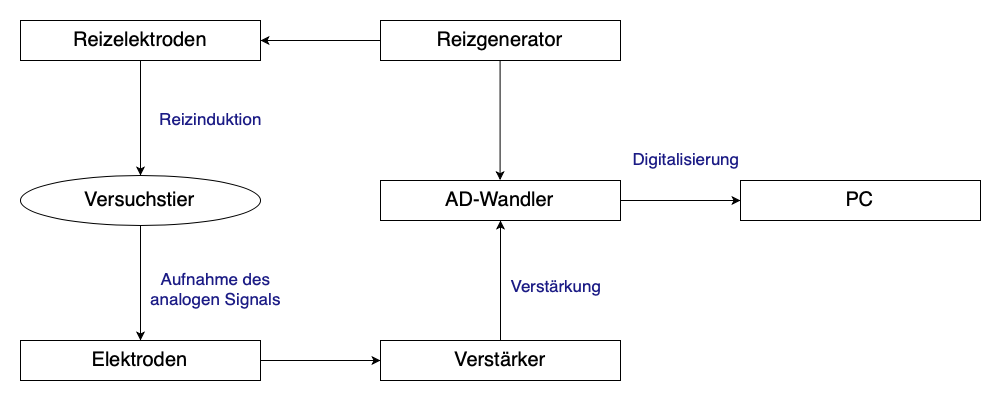
\includegraphics[width=1.3\textwidth]{schema}}
\caption{Die Abbildung zeigt einen schematischen Versuchsaufbau für den 1. - 3. Versuch. Gezeigt sind die verwendeten Komponenten und entlang der Pfeile ist der Informationsfluss zu erkennen. In blauer Schrift sind die Funktionen gekennzeichnet. }
\label{schema}
\end{figure}


\subsection{Versuchsdurchführung}

\subsubsection{Beobachtung der Lokomotion}
In diesem ersten Teil des Versuchs wurde der Regenwurm auf ein feuchtes Filterpapier gelegt und seine natürlichen Bewegungen beobachtet.\\
Anschließend wurde mit einem stumpfen Gegenstand mal das anteriore und mal das posteriere Ende gereizt um die jeweiligen Ausweich-, bzw. Meidereaktionen beobachten zu können. 

\subsubsection{Identifikation der Riesenfaser bei mechanischer Reizung}
Das Versuchstier wurde in der Wurmplatte fixiert (s. Versuchsaufbau) und ebenfalls mit einem stumpfen Gegenstand je fünf mal am anterioren und posterioren Ende gereizt. Dieses Mal wurde dabei eine differentielle Ableitung mit den Elektroden in der Wurmplatte durchgeführt und aufgezeichnet. Der Moment des Reizes wurde mit einem Keyboardmarker in Spike2 festgehalten. Zwischen zwei Reizen wurden dem Regenwurm je mindestens 30 Sekunden Ruhe gewährt.

\subsubsection{Bestimmung der Reizschwelle und der Fortleitungsgeschwindigkeit von MRF und LRF durch elektrische Reizung}
In diesem Versuchsteil wurde zusätzlich der Reizgenerator an die Wurmplatte angeschlossen, sodass eine elektrische Reizung des Wurm möglich war (siehe \ref{schema}). Die Reizelektroden wurden dafür am anterioren Ende des Wurmes angeschlossen. \\
Mit einer Reizdauern von $0.15$ms wurde der Wurm beginnend mit $0.5$V elektrisch gereizt.  Die Spannungsstärke wurde dann in Schritten von $0.5$V inkrementiert, bis zu einer maximalen Reizstärke von $10V$. \\
Die Reizstärke und der Zeitpunkt der Reizung wurden mittels Keyboardmarkern in Spike2 entsprechend markiert. \\
Der Zeitpunkt an dem zuerst ein Aktionspotential beobachtet werden konnte wurde protokolliert. \\



\textbf{Anmerkung}\\
Den folgenden Versuchsteile konnten wir am Versuchstag auf Grund von Zeitmangel durch Komplikationen bei den Messungen eider nicht mehr durchführen. Deshalb werden diese Experimente nur theoretisch beschrieben, fallen im Ergebnisteil weg und werden in der Diskussion auch theoretisch erörtert. 






\subsubsection{Bestimmung der Refraktärphasen bei elektrischer Reizung}
Hier hätte der gleiche Versuchsaufbau wie in 2.3.3 verwendet werden sollen. Der Wurm hätte mittels des Reizgenerators elektrisch gereizt werden sollen und gleichzeitig wäre eine differentielle Ableitung über die Elektroden erfolgt. \\
Diesmal wäre aber die Reizstärke konstant geblieben, während man dagegen aber eine Reizung mit der Einstellung \glqq Twin Pulse\grqq{} durchgeführt hätte, d.h. zwei kurz aufeinanderfolgende Reize. \\
Beginnend mit einem Delay (Abstand zwischen den beiden Reizen) von $20$ms hätte man den Regenwurm elektrisch gereizt. Diesen zeitlichen Abstand hätte man schrittweise dekrementiert, bis man nur noch ein einziges Aktionspotential beobachtet hätte. \\
Anschließend hätte man bei gleichbleibendem Delay die Reizstärke wieder schrittweise inkrementiert, bis man wieder ein zweites Aktionspotential beobachtet hätte. Zuletzt hätte man erneut den Delay bei gleichbleibender Reizstärke dekrementiert, bis wieder nur ein Aktionspotential zu beobachten gewesen wäre. 


\section{Ergebnisse}
Durch verschiedene Störfaktoren enthalten unsere Messungen leider viele Artefakte und sind zum Teil unvollständig.  \\

Screenshots für 2. : \\
$a4_1, a4_2, a6_1$ \\
$p3_3, p3_4, p4_2 $\\

Screenshots für 3. : \\
$g1_2, g2$ \\

\section{Diskussion}

\begin{thebibliography}{999}
\bibitem {lehninger} Nelson, David; Cox, Michael: Lehninger Biochemie. Springer Verlag, 2011.
\bibitem {zellbiologie} Karp, Gerald: Molekulare Zellbiologie. Springer Verlag, 2005.
\bibitem {haustiere} von Engelhardt, Wolfgang: Physiologie der Haustiere. Georg Thieme Verlag, 2010. 
\bibitem {physiologie} Schmidt, Robert; Lang, Florian; Heckmann, Manfred: Physiologie des Menschen, mit Pathopyhsiologie. Springer Medizin Verlag, 2010. 
\bibitem{koerperbau} \url{http://www.regenwuermer.info/regenwurm/regenwurm-koerperbau.php} \\Zugriff 18.01.2019 14:20 Uhr
\bibitem{skript} Skript: Erregungsleitung im Bauchmark des Regenwurms

\bibitem [Abbildung 1]{Abb1} \url{https://www.repetico.de/card-16616620}, \\Zugriff 17.01.2019 13:20 Uhr
\bibitem [Abbildung 2]{Abb2} Karp, Gerald: Molekulare Zellbiologie. Springer Verlag, 2005.
\bibitem [Abbildung 3]{bauchmark} \url{https://hypersoil.uni-muenster.de/1/02/26.htm}, \\Zugriff 18.01.2019 12:13 Uhr
\end{thebibliography}


\end{document}
